\documentclass[conference]{IEEEtran}
\usepackage{amsmath}
\usepackage{booktabs}
\usepackage{graphicx}
\usepackage{balance}
\usepackage[hidelinks]{hyperref}

\title{From Collisions to Recoveries: A Comparative Study of MARSALA Random Access}
\author{\IEEEauthorblockN{CESE4055 Group Project 2}
\IEEEauthorblockA{Ad Hoc and Sensor Networks}}

\begin{document}
\maketitle

\begin{abstract}
Satellite random access must recover packets when several users transmit in
the same time slot. This paper compares slotted ALOHA, contention resolution
diversity slotted ALOHA (CRDSA), and CRDSA with multi-replica decoding using
correlation-based localisation (MARSALA). We explain how repetition creates
both diversity and additional contention, then examine the effects of replica
count, signal-to-noise ratio (SNR), decoding threshold, and load. At an equal
arrival load of 75 packets per 100-slot frame, the model delivers 0.356,
0.502, and 0.750 packets per slot for slotted ALOHA, two-replica CRDSA, and
two-replica MARSALA, respectively. The receiver is an oracle-assisted concept
model, so these values illustrate mechanisms rather than predict physical-link
performance.
\end{abstract}

\begin{IEEEkeywords}
random access, slotted ALOHA, CRDSA, MARSALA, successive interference
cancellation, satellite communications
\end{IEEEkeywords}

\section{Introduction}
In a satellite return link, many terminals share a finite set of time slots.
Without scheduling, each terminal chooses its own transmission slot and
collisions are unavoidable. Slotted ALOHA treats a collision as a loss.
CRDSA instead sends several copies of each packet and uses successive
interference cancellation (SIC) to peel decoded packets from other slots
\cite{casini2007}. MARSALA retains the CRDSA transmitter but adds a receiver
step: it localises and combines collided replicas when SIC has no singleton
left to decode \cite{bui2015}.

The important question is not only which receiver delivers more packets, but
\emph{when} its extra complexity pays off. We compare the three receivers at
equal packet demand, study four adjustable parameters, and distinguish the
idealised model's predictions from a practical satellite link.

\section{Access and Decoding Mechanisms}
Let $N_s$ be the number of slots, $M$ the number of users, and $R$ the
replicas per packet. Packet arrival load and replica load are different:
\begin{equation}
U=\frac{M}{N_s}, \qquad G=\frac{MR}{N_s}=UR.
\label{eq:loads}
\end{equation}
Equal $G$ across different $R$ does not imply equal user demand. We hold
$U$ fixed for the parameter comparison.

\subsection{Slotted ALOHA}
Each user places one packet in one randomly chosen slot. A packet is received
only if no other user chooses that slot. For independent choices, the finite
frame throughput is
\begin{equation}
T_{\mathrm{SA}}=\frac{M}{N_s}\left(1-\frac{1}{N_s}\right)^{M-1}
\approx Ue^{-U}.
\label{eq:aloha}
\end{equation}
The large-frame peak is $1/e\approx0.368$ packets per slot. At $M=75$ and
$N_s=100$, (\ref{eq:aloha}) predicts approximately 0.355, close to the
measured 0.356.

\subsection{CRDSA and SIC}
CRDSA transmits $R$ copies in different slots. The receiver decodes a
singleton, cancels that packet's other copies, and repeats. A collision can
become a singleton after cancellation. If the remaining packets form a loop
with no singleton, this peeling process reaches a deadlock. Repetition helps
recovery but also raises $G$ and therefore creates more collisions.

\subsection{MARSALA at Deadlock}
MARSALA cross-correlates collided slot signals to locate replicas of one
packet, aligns their phases, combines them, and retries decoding. A newly
decoded packet can restart SIC. Under equal-power replicas and independent
interference, the approximate combined signal-to-interference-plus-noise ratio
(SINR) is
\begin{equation}
\mathrm{SINR}_{\mathrm{comb}}\simeq
\frac{R\rho}{1+(k-1)\rho},
\label{eq:sinr}
\end{equation}
where $\rho$ is per-replica SNR and $k$ is collision depth. The relation
explains why more copies or higher SNR can help, whereas deeper collisions or
a stricter decoding threshold can prevent recovery. It is an approximation,
not a complete link budget.

\section{Model and Comparison Method}
Each simulated frame contains $N_s=100$ slots and 256 complex samples per
slot. Replicas have independent random phases, small amplitude variation,
and additive Gaussian noise. A packet decodes when its modelled SINR exceeds
a threshold $\gamma$. The default is $R=2$, per-replica SNR $-2.2$~dB, and
$\gamma=0.61$. The controlled parameter study uses $M=75$ for every receiver
and averages 60 frames per point. Throughput is delivered packets divided by
$N_s$; frame loss is the undelivered fraction of the offered packets.

The fixed example frame illustrates the sequence: slotted ALOHA recovers
31/75 packets, CRDSA recovers 62/75, and MARSALA recovers 75/75. The 13
additional packets follow replica combination and renewed SIC. This example
is useful for explaining the algorithm; averaged results below describe the
parameter effects.

\begin{table}[t]
\caption{Throughput at Equal Packet Load $U=0.75$}
\label{tab:replicas}
\centering
\begin{tabular}{cccc}
\toprule
$R$ & Slotted ALOHA & CRDSA & MARSALA \\
\midrule
1 & 0.356 & 0.356 & 0.356 \\
2 & 0.356 & 0.502 & 0.750 \\
3 & 0.356 & 0.631 & 0.750 \\
4 & 0.356 & 0.428 & 0.750 \\
\bottomrule
\end{tabular}
\end{table}

\section{Parameter Effects}
\subsection{Number of Replicas}
Table~\ref{tab:replicas} shows diminishing returns from repetition. At
$R=2$, SIC raises throughput from the slotted ALOHA baseline of 0.356 to
0.502, and combining raises it to the offered-demand ceiling of 0.750. At
$R=3$, CRDSA improves to 0.631. At $R=4$, its throughput falls to 0.428:
the extra transmissions make slots more crowded. MARSALA stays at the
ceiling in this idealised study, so further copies use more channel resources
without delivering more packets. For $R=2$, the corresponding frame loss is
about 33\% under CRDSA and approximately zero under MARSALA.

\subsection{Per-Replica SNR}
With $R=2$, raising SNR from $-6$ to $-4$ to $-2.2$~dB increases MARSALA
throughput from 0.502 to 0.633 to 0.750 packets per slot. The ALOHA and
CRDSA curves barely move because the singleton decoding stand-in already
succeeds. SNR mainly determines whether a \emph{combined collision} crosses
the decoding threshold. Above $-2.2$~dB, throughput cannot rise further
because all offered packets are recovered in this experiment.

\subsection{Required Decoding SINR}
At the default SNR, increasing $\gamma$ from 0.61 to 0.8 to 1.0 reduces
MARSALA throughput from 0.750 to 0.640 to 0.502. At $\gamma=1.0$,
combining adds no recoveries over CRDSA. A stricter threshold is a stand-in
for a less capable code or a stronger reliability requirement. It excludes
borderline combined packets; the model does not quantify any coding gain or
error-rate benefit from that stricter requirement.

\begin{figure}[t]
\centering
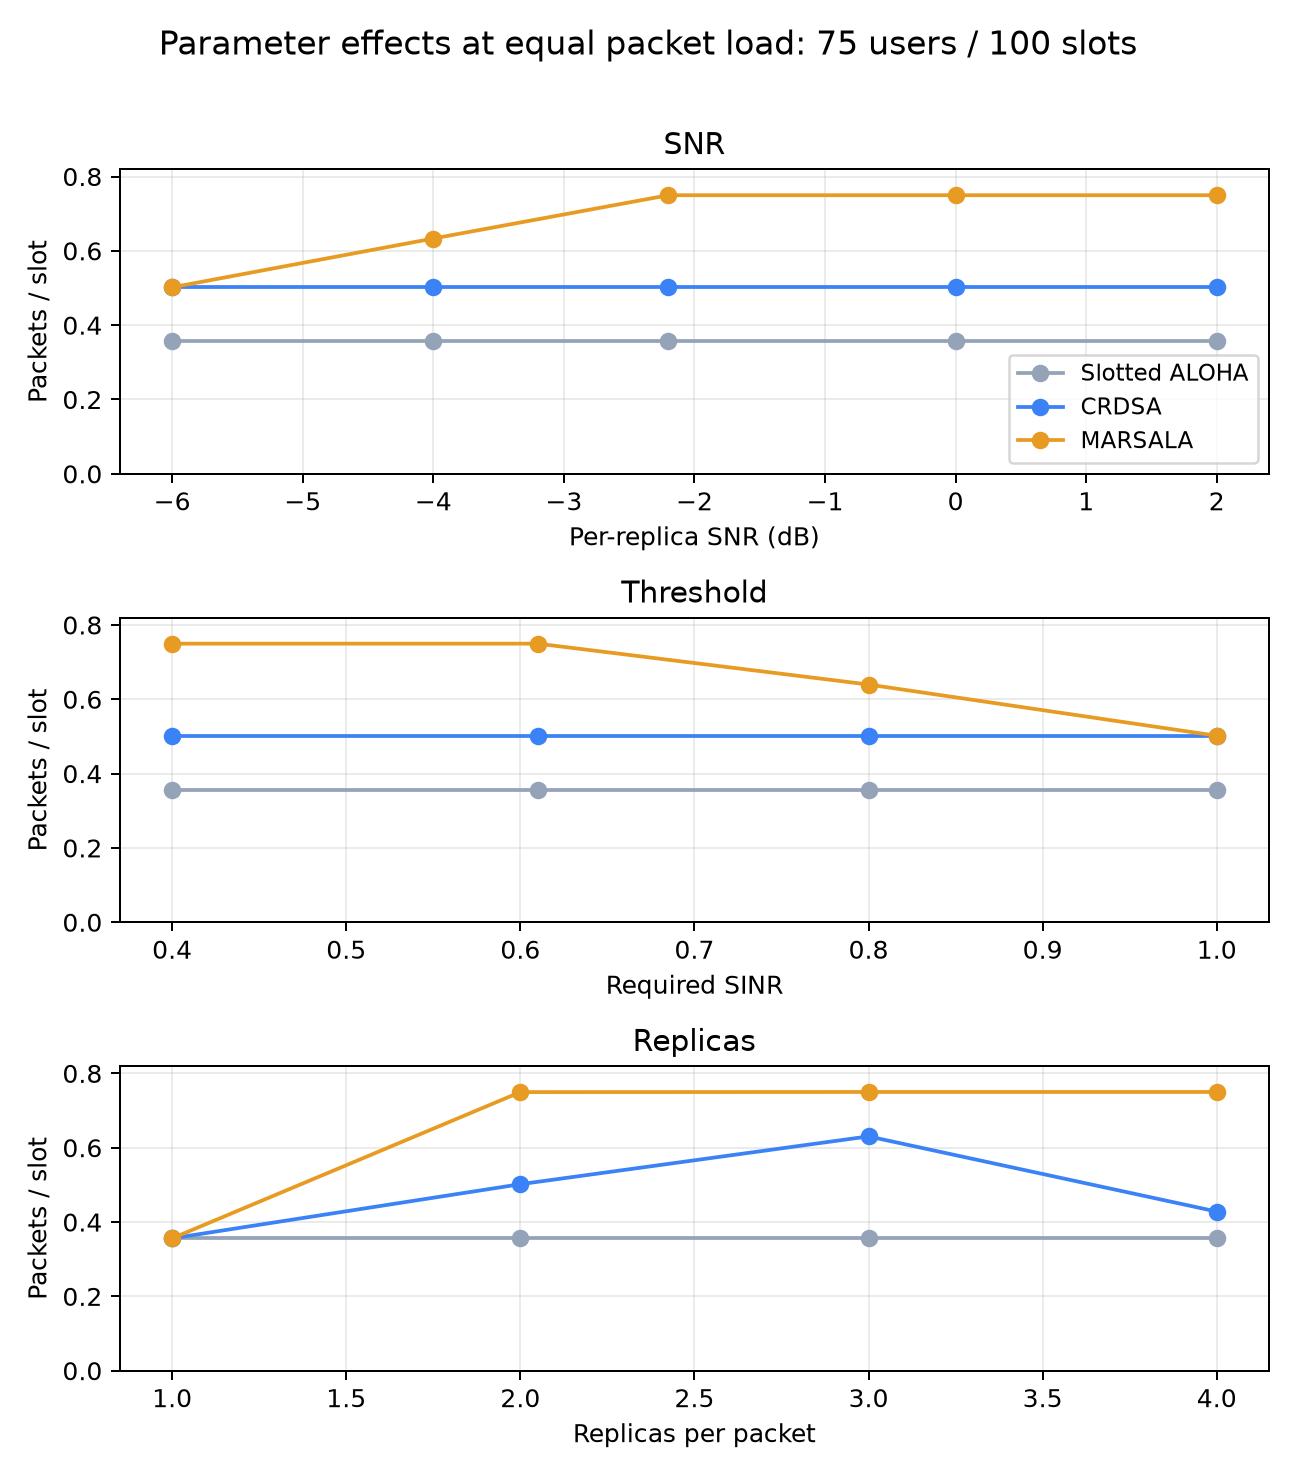
\includegraphics[width=\columnwidth]{results/parameter_effects.png}
\caption{Effect of SNR, decoding threshold, and replica count at equal
arrival load $U=0.75$. Each point averages 60 frames.}
\label{fig:parameters}
\end{figure}

\subsection{Offered Load}
As $U$ grows, singleton slots become rarer and ALOHA loss rises. SIC keeps
CRDSA useful beyond ALOHA's peak, while MARSALA can resolve some deadlocks.
At high occupancy, collision depth increases and the receiver must search
more candidate slots. Fig.~\ref{fig:throughput} plots delivered packets
against replica load $G$; curves for different $R$ should not be compared
as equal-demand experiments at the same horizontal coordinate.

\begin{figure}[t]
\centering
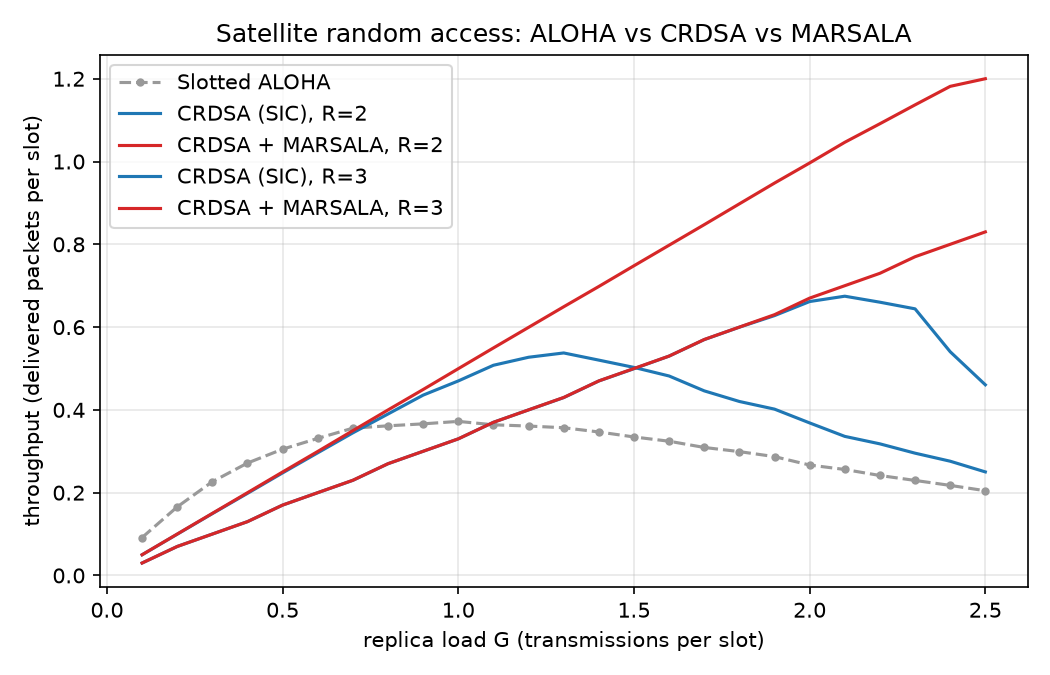
\includegraphics[width=\columnwidth]{results/throughput_vs_load.png}
\caption{Throughput versus replica load for the three receiver families.
The same $G$ corresponds to different user counts when $R$ differs.}
\label{fig:throughput}
\end{figure}

\section{Delay, Loss, and Complexity}
Undelivered packets in the delay experiment retry in new slots the next
frame and are dropped after 20 attempts. Mean delay is calculated only over
delivered packets, so it must be read alongside loss. At $G=2.5$ with
$R=2$, CRDSA's mean delay is 4.62 frames and MARSALA's is 1.04 frames in
this model. Unlocking a SIC cascade can therefore reduce retransmission
time. At equal demand $U=0.75$, the measured frame-loss fractions are
approximately 52.5\% for slotted ALOHA, 33.1\% for two-replica CRDSA,
and 0\% for two-replica MARSALA. Loss supplies essential context for the
mean delay, which excludes packets that were dropped.

MARSALA incurs extra receiver work: each deadlock requires slot
correlations, replica localisation, phase alignment, and combining. At
$G=2.5$ with $R=2$, this implementation averages about 11,353
correlations per frame.

\begin{figure}[t]
\centering
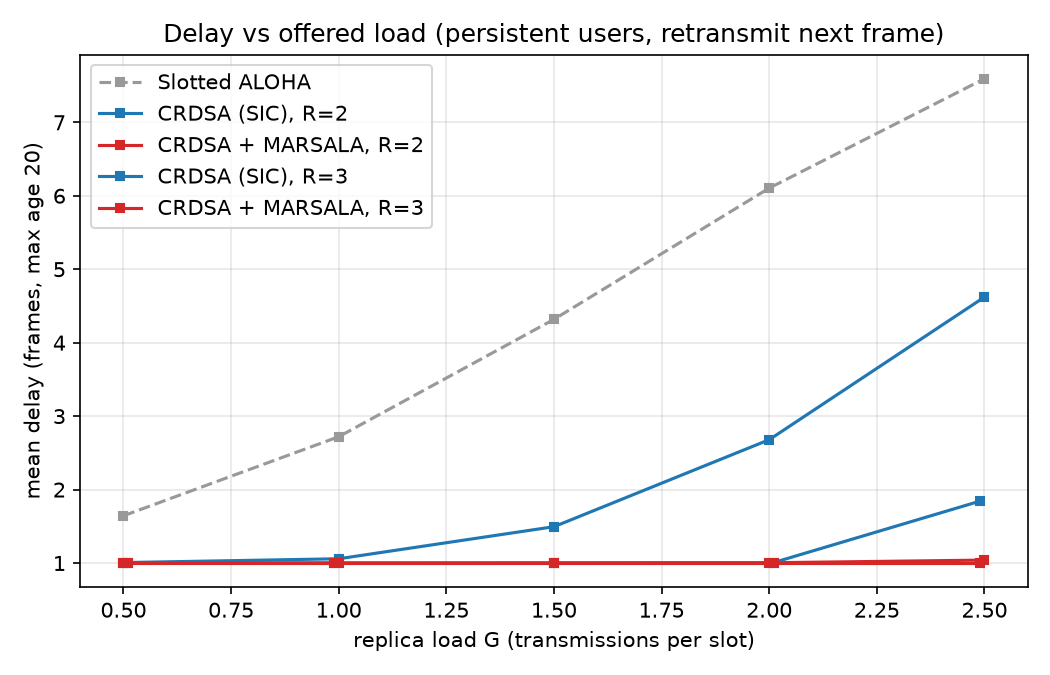
\includegraphics[width=\columnwidth]{results/delay_vs_load.png}
\caption{Mean delivered-packet delay under immediate next-frame
retransmission. Dropped packets are excluded from the mean.}
\label{fig:delay}
\end{figure}

\balance
\section{Scope and Limitations}
This is an \emph{oracle-assisted concept simulation}. The decoder reads
true slot occupancy, packet symbols, and amplitudes from the frame
generator. It does not perform blind packet identification, imperfect
channel estimation, a complete error-correcting code, or physical signal
subtraction. The modelled threshold is a surrogate for decoding success,
and the delay model omits feedback and propagation overhead. Thus the
figures illustrate how the mechanisms interact, not validated satellite-link
performance. In particular, the very high two-replica MARSALA throughput
under heavy load should not be quoted as a real-world prediction.

\section{Conclusion}
Slotted ALOHA loses collisions; CRDSA recovers some of them through
replication and SIC; MARSALA can combine collided replicas to restart SIC.
The controlled study shows that SNR and decoding threshold govern whether
combining helps, while replica count balances diversity against added
contention. The gain costs receiver correlations and depends on channel
knowledge that this concept model idealises. These tradeoffs, rather than
a single peak-throughput number, are the main lesson of the comparison.

\begin{thebibliography}{2}
\bibitem{casini2007} E. Casini, R. De Gaudenzi, and O. del Rio Herrero,
``Contention Resolution Diversity Slotted ALOHA (CRDSA): An Enhanced Random
Access Scheme for Satellite Access Packet Networks,'' \emph{IEEE Trans.
Wireless Commun.}, vol. 6, no. 4, pp. 1408--1419, 2007,
doi: \href{https://doi.org/10.1109/TWC.2007.348337}{10.1109/TWC.2007.348337}.
\bibitem{bui2015} H.-C. Bui, K. Zidane, J. Lacan, and M.-L. Boucheret,
``A Multi-Replica Decoding Technique for Contention Resolution Diversity
Slotted Aloha,'' in \emph{Proc. IEEE VTC-Fall}, 2015,
doi: \href{https://doi.org/10.1109/VTCFall.2015.7390798}{10.1109/VTCFall.2015.7390798}.
\end{thebibliography}
\end{document}
